% FreshTrack: IEEE conference paper (IEEEtran, conference mode).
% Build:  python paper/make_tables.py  &&  cd paper && latexmk -pdf freshtrack_ieee.tex
% Every number is a macro from generated/numbers.tex or a table from
% generated/tables.tex; do not type results by hand.
\documentclass[conference]{IEEEtran}
\IEEEoverridecommandlockouts
\usepackage{cite}
\usepackage{amsmath,amssymb}
\usepackage{graphicx}
\usepackage{booktabs}
\usepackage{url}
\usepackage[hidelinks]{hyperref}

% Generated by paper/make_tables.py - do not edit
\newcommand{\NImages}{14,682}
\newcommand{\NGroups}{1,279}
\newcommand{\ImgsPerGroup}{11.5}
\newcommand{\NTrain}{11,251}
\newcommand{\NVal}{1,643}
\newcommand{\NTest}{1,788}
\newcommand{\NTestGroups}{200}
\newcommand{\NaiveLeakPct}{100.0}
\newcommand{\NCross}{590}
\newcommand{\NNearOOD}{3,206}
\newcommand{\NExtDropped}{29}
\newcommand{\SplitSeed}{49}
\newcommand{\NSessions}{35}
\newcommand{\SessionSharePct}{97.7}
\newcommand{\NSingleSessionStrata}{4}
\newcommand{\NHeldOutStrata}{8}
\newcommand{\NSessTrain}{10,310}
\newcommand{\NSessVal}{2,050}
\newcommand{\NSessTest}{2,155}
\newcommand{\NSessExcluded}{167}
\newcommand{\NFilenameGroups}{1,622}
\newcommand{\NMixedClusters}{18}
\newcommand{\NMixedClusterImgs}{3,883}
\newcommand{\MaxClusterSize}{933}
\newcommand{\MtlFreshAcc}{98.3}
\newcommand{\MtlFreshAccStd}{0.1}
\newcommand{\MtlFreshFone}{98.3}
\newcommand{\MtlFreshFoneStd}{0.1}
\newcommand{\MtlTypeAcc}{99.8}
\newcommand{\MtlTypeAccStd}{0.2}
\newcommand{\MtlTypeFone}{99.8}
\newcommand{\MtlTypeFoneStd}{0.2}
\newcommand{\MtlCrossTypeAcc}{63.3}
\newcommand{\MtlCrossTypeAccStd}{2.6}
\newcommand{\MtlCrossShareFresh}{72.9}
\newcommand{\MtlCrossShareFreshStd}{2.1}
\newcommand{\MtlFreshEce}{1.4}
\newcommand{\MtlFreshEceStd}{0.3}
\newcommand{\MtlCpuMs}{22.3}
\newcommand{\MtlParams}{4.67}
\newcommand{\MtlGateTestIdAcceptRate}{95.7}
\newcommand{\MtlGateNearOODRejectRate}{91.5}
\newcommand{\MtlGateFarOODRejectRate}{96.8}
\newcommand{\MtlEnergyNearAuroc}{98.2}
\newcommand{\MtlEnergyFarAuroc}{99.4}
\newcommand{\MtlEntropyNearAuroc}{91.0}
\newcommand{\MtlEntropyFarAuroc}{95.8}
\newcommand{\MtlMspFreshNearAuroc}{91.1}
\newcommand{\MtlMspFreshFarAuroc}{95.8}
\newcommand{\FreshFreshAcc}{97.6}
\newcommand{\FreshFreshAccStd}{0.4}
\newcommand{\FreshFreshFone}{97.6}
\newcommand{\FreshFreshFoneStd}{0.4}
\newcommand{\FreshCrossShareFresh}{85.4}
\newcommand{\FreshCrossShareFreshStd}{4.3}
\newcommand{\FreshFreshEce}{1.7}
\newcommand{\FreshFreshEceStd}{0.1}
\newcommand{\FreshCpuMs}{24.6}
\newcommand{\FreshParams}{4.34}
\newcommand{\FreshGateTestIdAcceptRate}{90.9}
\newcommand{\FreshGateNearOODRejectRate}{61.1}
\newcommand{\FreshGateFarOODRejectRate}{75.7}
\newcommand{\FreshEntropyNearAuroc}{88.7}
\newcommand{\FreshEntropyFarAuroc}{93.7}
\newcommand{\FreshMspFreshNearAuroc}{88.7}
\newcommand{\FreshMspFreshFarAuroc}{93.7}
\newcommand{\TypeTypeAcc}{100.0}
\newcommand{\TypeTypeAccStd}{0.0}
\newcommand{\TypeTypeFone}{100.0}
\newcommand{\TypeTypeFoneStd}{0.0}
\newcommand{\TypeCrossTypeAcc}{62.7}
\newcommand{\TypeCrossTypeAccStd}{2.8}
\newcommand{\TypeCpuMs}{22.1}
\newcommand{\TypeParams}{4.34}
\newcommand{\TypeGateTestIdAcceptRate}{95.4}
\newcommand{\TypeGateNearOODRejectRate}{88.8}
\newcommand{\TypeGateFarOODRejectRate}{96.2}
\newcommand{\TypeEnergyNearAuroc}{97.2}
\newcommand{\TypeEnergyFarAuroc}{99.2}
\newcommand{\MnvFreshAcc}{98.5}
\newcommand{\MnvFreshAccStd}{0.4}
\newcommand{\MnvFreshFone}{98.5}
\newcommand{\MnvFreshFoneStd}{0.4}
\newcommand{\MnvTypeAcc}{99.7}
\newcommand{\MnvTypeAccStd}{0.4}
\newcommand{\MnvTypeFone}{99.8}
\newcommand{\MnvTypeFoneStd}{0.2}
\newcommand{\MnvCrossTypeAcc}{62.5}
\newcommand{\MnvCrossTypeAccStd}{1.8}
\newcommand{\MnvCrossShareFresh}{83.0}
\newcommand{\MnvCrossShareFreshStd}{3.8}
\newcommand{\MnvFreshEce}{1.1}
\newcommand{\MnvFreshEceStd}{0.2}
\newcommand{\MnvCpuMs}{16.7}
\newcommand{\MnvParams}{4.86}
\newcommand{\MnvGateTestIdAcceptRate}{93.5}
\newcommand{\MnvGateNearOODRejectRate}{86.4}
\newcommand{\MnvGateFarOODRejectRate}{97.3}
\newcommand{\MnvEnergyNearAuroc}{96.6}
\newcommand{\MnvEnergyFarAuroc}{99.3}
\newcommand{\MnvEntropyNearAuroc}{91.3}
\newcommand{\MnvEntropyFarAuroc}{95.1}
\newcommand{\MnvMspFreshNearAuroc}{91.3}
\newcommand{\MnvMspFreshFarAuroc}{95.1}
\newcommand{\NaiveFreshAcc}{100.0}
\newcommand{\NaiveFreshAccStd}{0.0}
\newcommand{\NaiveFreshFone}{100.0}
\newcommand{\NaiveFreshFoneStd}{0.0}
\newcommand{\NaiveTypeAcc}{100.0}
\newcommand{\NaiveTypeAccStd}{0.0}
\newcommand{\NaiveTypeFone}{100.0}
\newcommand{\NaiveTypeFoneStd}{0.0}
\newcommand{\NaiveCrossTypeAcc}{63.2}
\newcommand{\NaiveCrossTypeAccStd}{3.3}
\newcommand{\NaiveCrossShareFresh}{75.6}
\newcommand{\NaiveCrossShareFreshStd}{6.1}
\newcommand{\NaiveFreshEce}{0.0}
\newcommand{\NaiveFreshEceStd}{0.0}
\newcommand{\NaiveCpuMs}{22.4}
\newcommand{\NaiveParams}{4.67}
\newcommand{\NaiveGateTestIdAcceptRate}{94.2}
\newcommand{\NaiveGateNearOODRejectRate}{93.6}
\newcommand{\NaiveGateFarOODRejectRate}{97.5}
\newcommand{\NaiveEnergyNearAuroc}{98.1}
\newcommand{\NaiveEnergyFarAuroc}{99.4}
\newcommand{\NaiveEntropyNearAuroc}{93.9}
\newcommand{\NaiveEntropyFarAuroc}{95.0}
\newcommand{\NaiveMspFreshNearAuroc}{93.9}
\newcommand{\NaiveMspFreshFarAuroc}{95.0}
\newcommand{\SessFreshAcc}{84.9}
\newcommand{\SessFreshAccStd}{2.5}
\newcommand{\SessFreshFone}{83.7}
\newcommand{\SessFreshFoneStd}{2.9}
\newcommand{\SessTypeAcc}{98.5}
\newcommand{\SessTypeAccStd}{0.5}
\newcommand{\SessTypeFone}{97.8}
\newcommand{\SessTypeFoneStd}{1.4}
\newcommand{\SessCrossTypeAcc}{58.7}
\newcommand{\SessCrossTypeAccStd}{5.5}
\newcommand{\SessCrossShareFresh}{72.1}
\newcommand{\SessCrossShareFreshStd}{13.1}
\newcommand{\SessFreshEce}{12.2}
\newcommand{\SessFreshEceStd}{2.4}
\newcommand{\SessCpuMs}{21.6}
\newcommand{\SessParams}{4.67}
\newcommand{\SessGateTestIdAcceptRate}{95.6}
\newcommand{\SessGateNearOODRejectRate}{69.5}
\newcommand{\SessGateFarOODRejectRate}{90.2}
\newcommand{\SessEnergyNearAuroc}{93.9}
\newcommand{\SessEnergyFarAuroc}{98.4}
\newcommand{\SessEntropyNearAuroc}{78.7}
\newcommand{\SessEntropyFarAuroc}{88.1}
\newcommand{\SessMspFreshNearAuroc}{78.7}
\newcommand{\SessMspFreshFarAuroc}{88.1}
\newcommand{\HistGroupedFreshAcc}{86.3}
\newcommand{\HistGroupedTypeAcc}{80.0}
\newcommand{\HistNaiveFreshAcc}{94.0}
\newcommand{\HistNaiveTypeAcc}{96.6}
\newcommand{\MtlSzeroFreshAcc}{98.3}
\newcommand{\MtlSzeroFreshCI}{[96.4, 99.6]}
\newcommand{\MtlSzeroTypeAcc}{99.9}
\newcommand{\MtlSzeroTypeCI}{[99.6, 100.0]}
\newcommand{\DeployGateAccept}{94.5}
\newcommand{\DeployGateNear}{77.1}
\newcommand{\DeployGateFar}{94.2}
\newcommand{\MnvGateNearMin}{77.1}
\newcommand{\MnvGateNearMax}{91.4}
\newcommand{\MtlCrossShareFreshExact}{72.9}
\newcommand{\MnvCrossShareFreshExact}{83.0}
\newcommand{\EpochsMin}{5}
\newcommand{\EpochsMax}{10}
\newcommand{\SessHeldAppleStale}{97.4}
\newcommand{\SessHeldBitterGourdFresh}{99.2}
\newcommand{\SessHeldBitterGourdStale}{100.0}
\newcommand{\SessHeldCapsicumFresh}{26.6}
\newcommand{\SessHeldCapsicumStale}{6.9}
\newcommand{\SessHeldOrangeFresh}{99.9}
\newcommand{\SessHeldTomatoFresh}{55.2}
\newcommand{\SessHeldTomatoStale}{99.0}
\newcommand{\SessStrataGroupedFreshAcc}{98.9}
\newcommand{\SessStrataHeldFreshAcc}{87.0}
\newcommand{\SessStrataGroupedTypeAcc}{99.8}
\newcommand{\SessStrataHeldTypeAcc}{91.5}
\newcommand{\NSessCommonStrata}{6}

\IfFileExists{generated/app_numbers.tex}{% Generated by paper/make_tables.py from results/mobile_metrics.json - do not edit
\newcommand{\AppApkArm}{52.3}
\newcommand{\AppApkArmSeven}{44.9}
\newcommand{\AppOrtMb}{19.2}
\newcommand{\AppModelMb}{19.4}
\newcommand{\AppParityN}{40}
\newcommand{\AppParityMaxDiff}{0.27}
\newcommand{\AppPipeMs}{137--142}
\newcommand{\AppScanMs}{440}
\newcommand{\AppColdMs}{2.2}
\newcommand{\AppRamIdle}{85}
\newcommand{\AppRamLoaded}{169}
\newcommand{\AppRamPeak}{327}
\newcommand{\AppScanKb}{46}
}{}

\begin{document}

\title{Leakage-Aware Multi-Task Recognition of Produce Freshness and Type for Low-Cost Mobile Deployment}

\author{
\IEEEauthorblockN{Yashash Mathur}
\IEEEauthorblockA{\textit{RV Institute of Technology and Management}\\
Bengaluru, India\\
yashashgdg@gmail.com}
\and
\IEEEauthorblockN{Utsav Upadhyay}
\IEEEauthorblockA{\textit{RV Institute of Technology and Management}\\
Bengaluru, India}
\and
\IEEEauthorblockN{Aditya Prakash}
\IEEEauthorblockA{\textit{RV Institute of Technology and Management}\\
Bengaluru, India}
\and
\IEEEauthorblockN{Shresth Modi}
\IEEEauthorblockA{\textit{RV Institute of Technology and Management}\\
Bengaluru, India}
}

\maketitle

\begin{abstract}
Public fresh/rotten produce datasets are routinely reported with accuracies
close to 100\%. We show that, for a widely used Kaggle dataset, much of this
figure is an artefact of how the data are split and how the data were
collected. Its \NImages{} images derive from only \NGroups{} source
photographs taken in \NSessions{} (file-name-inferred) capture sessions. A per-file split places a
sibling of \NaiveLeakPct\% of test images in training, and an EfficientNet-B0
then scores \NaiveFreshAcc\% on freshness. Grouping copies by source photo
gives \MtlFreshAcc\%, yet \SessionSharePct\% of test images still share a
capture session with training. Holding out whole sessions lowers freshness
accuracy to \SessFreshAcc\%, and expected calibration error grows from
\MtlFreshEce\% to \SessFreshEce\%. The loss is concentrated in produce types
whose fresh and stale photographs came from different cameras or messaging
apps: on an unseen session of stale capsicum the model is correct on only
\SessHeldCapsicumStale\% of images, suggesting it has partly learned the
acquisition source rather than freshness. On the photo-grouped split, joint
training of freshness and produce type shows no difference from separate
single-task models that three seeds can resolve, and MobileNetV3-Large matches EfficientNet-B0 (\MnvFreshAcc\% vs.
\MtlFreshAcc\%) at \MnvCpuMs{}\,ms CPU latency. An energy-score gate on the
produce-type head rejects \MnvGateFarOODRejectRate\% of non-produce images and
\MnvGateNearOODRejectRate\% of unseen produce while accepting
\MnvGateTestIdAcceptRate\% of in-distribution images; produce-type accuracy on
an external dataset is only \MnvCrossTypeAcc\%. We release splits and code, and
argue that shelf life and quality grade, which have no ground truth in these
datasets, should not be presented as learned outputs.

\end{abstract}

\begin{IEEEkeywords}
food quality, freshness classification, data leakage, multi-task learning,
out-of-distribution detection, on-device inference
\end{IEEEkeywords}

%===========================================================================
\section{Introduction}
In informal markets, fruit and vegetables are usually sorted by eye. A phone
app that flags stale produce from a single photo would be a cheap aid for
vendors and shoppers, and public datasets of fresh and rotten (or stale)
produce have turned the idea into a popular benchmark. Reported accuracies sit
close to 100\%~\cite{noisyvit2025}.

We were suspicious of those numbers for a simple reason. Several of the most
widely used Kaggle releases ship \emph{pre-augmented} images: the same
photograph appears many times, rotated, flipped, shifted or sprinkled with
noise. Split such a dataset at random, file by file, and near-copies of a test
image end up in the training set. This is the textbook form of leakage
described by Kaufman \emph{et al.}~\cite{kaufman2012leakage}, and Kapoor and
Narayanan~\cite{kapoor2023leakage} show how widespread it is in applied
machine learning.

This paper asks how much of the reported performance survives once that leakage
is removed, and then pushes one level further, to the sessions in which the
photographs were taken. We make four contributions.
\begin{enumerate}
\item A leakage audit of the Kaggle ``Fresh and Stale Images of Fruits and
Vegetables'' dataset~\cite{kaggle_fresh_stale}. Its \NImages{} images collapse
into \NGroups{} near-duplicate clusters (\NFilenameGroups{} by file name
alone), and a per-file split puts a sibling of \NaiveLeakPct\% of test images
into training. A held-out-session analysis then shows that part of the
remaining accuracy depends on how and when the photographs were taken. We
release both splits.
\item A controlled comparison of multi-task and single-task networks with
identical backbones, and of EfficientNet-B0~\cite{tan2019efficientnet} and
MobileNetV3-Large~\cite{howard2019mobilenetv3}, over three seeds.
\item An evaluation of post-hoc out-of-distribution (OOD) gates that reject
photos of unsupported produce and of things that are not produce at all.
\item An Android app that runs the model entirely on the phone and shows
quality grade and remaining shelf life, which no available dataset annotates,
only as clearly labelled estimates.
\end{enumerate}

%===========================================================================
\section{Related Work}
\textbf{Freshness classification.} Classifiers trained on public fresh/rotten
datasets routinely report accuracies in the high 90s. Transfer-learned AlexNet
reaches 99.8\% on one such dataset~\cite{amin2023freshness}, and a multi-task
ResNet ensemble predicts freshness and fruit type together at 98.5\% and
97.4\%~\cite{kang2022ensemble}. The closest work to ours is Multi-Task
NoisyViT~\cite{noisyvit2025}, which reports 99.85\% on the same Fresh/Stale
dataset using random 60/20/20 splits; the only deduplication it describes is MD5
hashing, applied when building a merged Freshness44 set. In~\cite{amin2023freshness}
the images are rotation-augmented \emph{before} a random 80/10/10 split. None of
these papers keeps augmented or near-duplicate copies of a photograph on one
side of the split, and we could not find a freshness study that measures how
much this matters.

\textbf{Shelf-life estimation.} Remaining shelf life cannot be learned without
measuring it. Datasets that follow produce over time until it spoils do
exist~\cite{fruqdb2022}, and a recent CNN+DeiT study~\cite{shelflife2026arxiv}
forecasts spoilage with a symmetric mean absolute percentage error above 40\%.
Our dataset has no such measurements, so we do not try to learn shelf life.

\textbf{Multi-task learning.} A shared representation can help related
tasks~\cite{caruana1997multitask,ruder2017overview}, but only when the tasks
really are related. We test this directly.

\textbf{OOD detection.} Maximum softmax probability (MSP)~\cite{hendrycks2017baseline}
and the energy score~\cite{liu2020energy} need no retraining, which makes them
easy to run on a phone.

\textbf{Leakage.} Kaufman \emph{et al.}~\cite{kaufman2012leakage} formalise
leakage in data mining, and Kapoor and Narayanan~\cite{kapoor2023leakage} show
how often it inflates published results, with samples duplicated across splits
among the causes.

%===========================================================================
\section{Data and Leakage Audit}
\subsection{Datasets}
\textbf{Main set.} The Kaggle ``Fresh and Stale Images of Fruits and
Vegetables'' dataset~\cite{kaggle_fresh_stale} has \NImages{} images of six
produce types: apple, banana, bitter gourd, capsicum, orange and tomato. Each
image is labelled fresh or stale by the folder it sits in, and we use both
labels as ground truth.

\textbf{External set.} We use the Kaggle ``Fruit and Vegetable Image
Recognition'' dataset~\cite{kaggle_fruit_veg_recognition} (36 classes, no
freshness labels) for evaluation only. Its \NCross{} images of apple, banana,
orange, tomato, capsicum and bell pepper form a cross-dataset test of produce
type, and the \NNearOOD{} images of its other classes form a near-OOD set. We
drop \NExtDropped{} external images that are near-duplicates of main-set images.

\textbf{Far-OOD set.} We draw 2,000 CIFAR-10 test images~\cite{krizhevsky2009cifar}
at random and upsample them to the model's input size.

\subsection{Leakage and the grouped split}
\begin{sloppypar}
The file names tell you how each image was made. Prefixes such as
\texttt{rotated\_by\_15\_}, \texttt{saltandpepper\_}, \texttt{translation\_},
\texttt{vertical\_flip\_} and \texttt{Copy of}, and suffixes such as
\texttt{.jpg\_0\_4456.jpg}, mark augmented copies of a source photo. We strip
these markers, map every file back to its source name, and group files that
share a source within a produce type (\NFilenameGroups{} groups). We then
compute a 64-bit difference hash of every image and merge groups whose images
are within 2 bits of each other, again only within a produce type, because
low-texture images of different produce otherwise collide. The result is
\NGroups{} clusters.
\end{sloppypar}

Merging is transitive, so a single chance match can join two different
photographs. \NMixedClusters{} clusters (\NMixedClusterImgs{} images) contain
both fresh and stale images, and the largest holds \MaxClusterSize{} images.
Over-merging cannot leak test images into training; it only makes the split
coarser. For that reason we call the units clusters rather than photographs.

We assign whole clusters to train, validation and test with stratified group
$k$-fold sampling. Some photo sessions contain hundreds of copies, so a single
random draw can starve a class. We therefore try 50 seeds and keep the split
whose per-stratum validation and test shares are closest to 15\% (seed
\SplitSeed{}). It has \NTrain{}/\NVal{}/\NTest{} images and \NTestGroups{}
independent test clusters (Table~\ref{tab:split}). For comparison we also draw a
per-file split with the same proportions; under it, \NaiveLeakPct\% of test
images have a sibling in training.

% Generated by paper/make_tables.py - do not edit
\begin{table}[t]
\centering
\caption{Grouped split: images per produce type, freshness and split.}
\label{tab:split}
\footnotesize
\setlength{\tabcolsep}{3pt}
\begin{tabular}{lrrrrrr}
\toprule
 & \multicolumn{2}{c}{Train} & \multicolumn{2}{c}{Val} & \multicolumn{2}{c}{Test} \\
\cmidrule(lr){2-3}\cmidrule(lr){4-5}\cmidrule(lr){6-7}
Type & Fresh & Stale & Fresh & Stale & Fresh & Stale \\
\midrule
Apple & 1,165 & 1,741 & 300 & 307 & 228 & 294 \\
Banana & 1,219 & 1,036 & 158 & 223 & 204 & 208 \\
Bitter gourd & 246 & 294 & 41 & 0 & 40 & 63 \\
Capsicum & 836 & 860 & 31 & 41 & 123 & 0 \\
Orange & 1,033 & 1,144 & 228 & 192 & 205 & 259 \\
Tomato & 941 & 736 & 40 & 82 & 0 & 164 \\
\bottomrule
\end{tabular}
\end{table}
\begin{table}[t]
\centering
\caption{Accuracy (\%) under a per-file split versus the grouped split. $\Delta$ = inflation caused by leakage.}
\label{tab:leak}
\footnotesize
\setlength{\tabcolsep}{2.5pt}
\begin{tabular}{lcccccc}
\toprule
 & \multicolumn{3}{c}{Freshness} & \multicolumn{3}{c}{Produce type} \\
\cmidrule(lr){2-4}\cmidrule(lr){5-7}
Model & Per-file & Grouped & $\Delta$ & Per-file & Grouped & $\Delta$ \\
\midrule
HSV hist.+LR & 94.0 & 86.3 & +7.7 & 96.6 & 80.0 & +16.6 \\
B0 multi-task & 100.0 & 98.3 & +1.7 & 100.0 & 99.8 & +0.2 \\
\bottomrule
\end{tabular}
\end{table}
\begin{table*}[t]
\centering
\caption{Test results on the photo-grouped split (capture sessions are still shared with training), mean $\pm$ std over three seeds (\%). CPU latency: batch 1, 4 threads, median of 200 interleaved runs.}
\label{tab:main}
\begin{tabular}{lcccccc}
\toprule
Model & Fresh acc. & Fresh macro-F1 & Type acc. & Type macro-F1 & Params (M) & CPU (ms) \\
\midrule
EfficientNet-B0, multi-task & 98.3 $\pm$ 0.1 & 98.3 $\pm$ 0.1 & 99.8 $\pm$ 0.2 & 99.8 $\pm$ 0.2 & 4.67 & 22.3 \\
EfficientNet-B0, freshness only & 97.6 $\pm$ 0.4 & 97.6 $\pm$ 0.4 & -- & -- & 4.34 & 24.6 \\
EfficientNet-B0, type only & -- & -- & 100.0 $\pm$ 0.0 & 100.0 $\pm$ 0.0 & 4.34 & 22.1 \\
MobileNetV3-L, multi-task & 98.5 $\pm$ 0.4 & 98.5 $\pm$ 0.4 & 99.7 $\pm$ 0.4 & 99.8 $\pm$ 0.2 & 4.86 & 16.7 \\
HSV histogram + LR & 86.3 & 86.2 & 80.0 & 76.0 & -- & -- \\
\bottomrule
\end{tabular}
\end{table*}
\begin{table*}[t]
\centering
\caption{Out-of-distribution detection (\%, mean $\pm$ std over three seeds). Near-OOD: unseen produce classes from an external dataset; far-OOD: CIFAR-10 test images. Higher AUROC and lower FPR@95\%TPR are better.}
\label{tab:ood}
\begin{tabular}{lcccc}
\toprule
 & \multicolumn{2}{c}{Near-OOD (\NNearOOD{} images)} & \multicolumn{2}{c}{Far-OOD (2,000 images)} \\
\cmidrule(lr){2-3}\cmidrule(lr){4-5}
Score & AUROC & FPR@95 & AUROC & FPR@95 \\
\midrule
\multicolumn{5}{l}{\textit{EfficientNet-B0, multi-task}} \\
\quad Neg. entropy, freshness (v1 gate) & 91.0 $\pm$ 2.5 & 37.7 $\pm$ 8.7 & 95.8 $\pm$ 0.8 & 25.8 $\pm$ 7.8 \\
\quad MSP, freshness & 91.1 $\pm$ 2.5 & 37.7 $\pm$ 8.7 & 95.8 $\pm$ 0.8 & 25.8 $\pm$ 7.8 \\
\quad MSP, produce type & 97.8 $\pm$ 0.4 & 8.8 $\pm$ 1.8 & 98.9 $\pm$ 0.4 & 3.7 $\pm$ 2.6 \\
\quad Energy, produce type & 98.2 $\pm$ 0.4 & 7.7 $\pm$ 2.0 & 99.4 $\pm$ 0.2 & 2.7 $\pm$ 1.5 \\
\multicolumn{5}{l}{\textit{MobileNetV3-L, multi-task}} \\
\quad Neg. entropy, freshness (v1 gate) & 91.3 $\pm$ 1.6 & 42.9 $\pm$ 4.6 & 95.1 $\pm$ 1.5 & 32.3 $\pm$ 11.8 \\
\quad MSP, freshness & 91.3 $\pm$ 1.6 & 42.9 $\pm$ 4.6 & 95.1 $\pm$ 1.5 & 32.3 $\pm$ 11.8 \\
\quad MSP, produce type & 96.0 $\pm$ 1.2 & 19.1 $\pm$ 7.2 & 98.3 $\pm$ 0.6 & 6.8 $\pm$ 4.4 \\
\quad Energy, produce type & 96.6 $\pm$ 1.6 & 15.4 $\pm$ 8.4 & 99.3 $\pm$ 0.5 & 3.6 $\pm$ 3.1 \\
\bottomrule
\end{tabular}
\end{table*}


%===========================================================================
\section{Method}
\subsection{Model}
A timm~\cite{wightman2019timm} backbone pretrained on ImageNet~\cite{deng2009imagenet}
(EfficientNet-B0 or MobileNetV3-Large) produces a pooled feature vector, and each
task gets its own small head: dropout 0.3, a 256-unit layer with ReLU, dropout
0.2 and a linear output, with two classes for freshness and six for produce
type. The multi-task loss is the mean of the two cross-entropy losses. The
single-task baselines use the same backbone and head with one task.

\subsection{Heuristic attributes}
No dataset we could find contains graded quality or measured shelf life, so we
learn neither. The app still shows both as rough guides, derived from the
predicted $p=P(\text{fresh})$: grade A if $p\ge0.85$, B if $p\ge0.5$ and C
otherwise, and an indicative shelf life of $d_t\,p$ days, where $d_t$ is a
room-temperature reference for produce type $t$. Both fields are labelled as
estimates, and we make no accuracy claim about them.

\subsection{OOD gate}
We compare four post-hoc scores: the negative entropy of the freshness head,
which was the gate used by an earlier version of the system; the MSP of the
freshness head; the MSP of the produce-type head~\cite{hendrycks2017baseline};
and the energy score $\log\sum_k e^{z_k}$ over the produce-type logits, i.e.\ the
negative free energy at temperature 1~\cite{liu2020energy}. The deployed gate
uses the energy score. Its threshold accepts 95\% of validation images and is
stored with the model.

\subsection{Training and evaluation}
Images are resized to $224\times224$ and normalised with ImageNet statistics.
During training we apply random resized crops (scale 0.8--1), horizontal and
vertical flips, 90\textdegree{} rotations, colour jitter, Gaussian noise and
coarse dropout. We use AdamW~\cite{loshchilov2019adamw} with a learning rate of
$3\times10^{-4}$, weight decay $10^{-4}$ and batch size 64. The first epoch runs
at 10\% of the base learning rate, followed by cosine decay. Training uses mixed
precision and gradient clipping at 1.0, and stops early on validation loss
(patience 3) after at most 10 epochs; in practice runs stopped after
\EpochsMin--\EpochsMax{} epochs. Every configuration is trained with seeds 0, 1
and 2, and we report the mean and standard deviation. Calibration is measured
with the expected calibration error (ECE, 15 bins)~\cite{guo2017calibration}.
Images from one cluster are not independent, so for a single run we report a
95\% confidence interval from 1,000 bootstrap resamples of test clusters rather
than images~\cite{efron1994bootstrap}. As a floor we train a logistic-regression
classifier on $8\times8\times8$ HSV colour histograms.

Training ran on one NVIDIA RTX 4060 Laptop GPU (8 GB). Latency is measured on
an Intel Core i7-14700HX with 4 threads and batch size 1, as the median of 200
runs interleaved across all models so that background load affects them
equally. We used Python 3.13, PyTorch 2.12, timm 1.0.24, PyTorch Lightning 2.6.1
and Albumentations 2.0.8. Code, splits and per-run logs are available at
\url{https://github.com/mathuryashash/FreshTrack_AI}.

%===========================================================================
\section{Results}
\subsection{Leakage from augmented copies}
Table~\ref{tab:leak} and Fig.~\ref{fig:leak} compare the per-file and grouped
protocols. Under the per-file split every EfficientNet-B0 seed classifies every
test image correctly (\NaiveFreshAcc\% freshness, \NaiveTypeAcc\% type). The
grouped split lowers this to \MtlFreshAcc\% and \MtlTypeAcc\%. The effect is
larger for the colour-histogram baseline, whose freshness accuracy drops from
\HistNaiveFreshAcc\% to \HistGroupedFreshAcc\% and type accuracy from
\HistNaiveTypeAcc\% to \HistGroupedTypeAcc\%: the per-file split lets even a
model with no spatial features look almost as good as a deep network, which
hides how much of the task the CNN actually solves.

\begin{figure}[t]
\centering
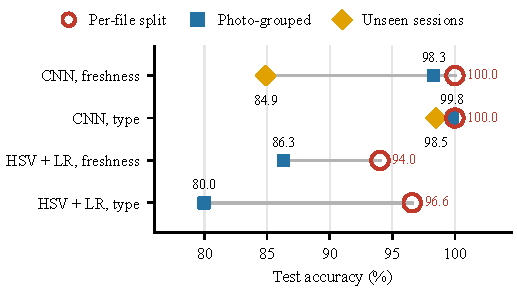
\includegraphics[width=\columnwidth]{figures/leakage.pdf}
\caption{Test accuracy under the per-file and grouped splits.}
\label{fig:leak}
\end{figure}

\subsection{Session-level dependence}
Grouping by source photo does not make test images independent of training.
File names indicate only \NSessions{} capture sessions (a capture date or
camera series within a class; we infer them from file-name patterns), and \SessionSharePct\% of grouped-split test images
come from a session that also contributes training images; \NSingleSessionStrata{}
of the 12 produce/freshness strata consist of a single session. For the
\NHeldOutStrata{} strata with more than one session we built a held-out-session
split (\NSessTrain{}/\NSessVal{}/\NSessTest{} images) in which each such stratum
contributes one entire, unseen session to the test set. We drop the
\NSessExcluded{} training images that are augmented copies (same file-name
source) or near-duplicates (dHash within 2 bits) of a test image; no remaining
training image is within 2 bits of a test image. Clusters from the grouped
split may still span train and test here, because chained merging links
different photographs of the same session, which is exactly the dependence
this protocol probes.

On this split freshness accuracy is \SessFreshAcc\% (vs.\ \MtlFreshAcc\% on the
grouped split), while produce-type accuracy stays at \SessTypeAcc\%, and the
freshness ECE rises from \MtlFreshEce\% to \SessFreshEce\%: the model becomes
confidently wrong. Table~\ref{tab:session} breaks this down by stratum. On the
\NSessCommonStrata{} strata that also occur in the grouped test, accuracy falls
only from \SessStrataGroupedFreshAcc\% to \SessStrataHeldFreshAcc\%; apple,
bitter gourd and orange sessions transfer almost perfectly. The failures are
capsicum (\SessHeldCapsicumFresh\% on an unseen fresh session,
\SessHeldCapsicumStale\% on an unseen stale session) and fresh tomato
(\SessHeldTomatoFresh\%). In both cases the held-out session's capture source
appears in training only with the opposite label: every stale capsicum left in
training is a WhatsApp-compressed photograph, while every camera (IMG-series)
capsicum in training is fresh, so camera photographs of stale capsicums are
called fresh; likewise, all IMG-series tomatoes in training are stale, and the
held-out IMG-series fresh tomatoes are often called stale. This pattern is consistent with
the network having partly learned the acquisition source, a shortcut that
per-file and per-photo splits cannot reveal because \SessionSharePct\% of their
test images share a capture session with training images.

\subsection{Multi-task versus single-task learning and backbones}
Table~\ref{tab:main} reports the grouped-split results. The multi-task
EfficientNet-B0 reaches \MtlFreshAcc\% freshness and \MtlTypeAcc\% type
accuracy, against \FreshFreshAcc\% and \TypeTypeAcc\% for the single-task
networks. The differences are below one percentage point and point in
opposite directions (freshness favours the multi-task model, type the
single-task one); three seeds cannot resolve them, so we find no evidence that
joint training helps or hurts, while one shared network halves inference cost. MobileNetV3-Large matches
EfficientNet-B0 (\MnvFreshAcc\% and \MnvTypeAcc\%) with \MnvParams{}\,M
parameters and \MnvCpuMs{}\,ms CPU latency against \MtlCpuMs{}\,ms, and is the
model we deploy. For a single seed-0 run the 95\% group-bootstrap interval of
freshness accuracy is \MtlSzeroFreshCI{}\%, reflecting that the \NTestGroups{}
test groups, not the \NTest{} images, are the independent units.

\subsection{Cross-dataset produce type}
On \NCross{} external images of five of the six produce types (bell pepper is
mapped to capsicum; there is no bitter gourd), type accuracy is only
\MnvCrossTypeAcc\% (MobileNetV3) and \MtlCrossTypeAcc\% (EfficientNet-B0),
compared with about 99\% in-domain. The external set has no freshness labels;
MobileNetV3 calls \MnvCrossShareFreshExact\% of these retail-style photos fresh
and EfficientNet-B0 \MtlCrossShareFreshExact\%, which is plausible but not an
accuracy.

\subsection{Out-of-distribution gate}
Table~\ref{tab:ood} compares post-hoc scores. Scores computed on the six-way
produce-type head separate in- from out-of-distribution images much better
than scores on the binary freshness head (near-OOD AUROC
\MnvEnergyNearAuroc\% for energy on the type head vs.\ \MnvMspFreshNearAuroc\%
for MSP on the freshness head). For a two-class head, entropy is a monotone
function of MSP, so entropy ranks inputs exactly like MSP. The previous
version of the system rejected an input when freshness entropy exceeded
1.5 bits or its maximum probability fell below 0.3; for a two-class head
neither condition can occur (entropy is at most 1 bit and the maximum
probability at least 0.5), so that gate never fired. With the threshold set at
95\% validation TPR, the MobileNetV3 energy gate, averaged over three seeds,
accepts \MnvGateTestIdAcceptRate\% of in-distribution test images and rejects
\MnvGateFarOODRejectRate\% of CIFAR-10 images but only
\MnvGateNearOODRejectRate\% of unseen produce (\MnvGateNearMin--\MnvGateNearMax\%
across seeds; the deployed seed: \DeployGateAccept\%, \DeployGateFar\% and
\DeployGateNear\%). A photo of an unsupported vegetable is the hard case.


%===========================================================================
\section{Deployment}
\IfFileExists{sections/deployment.tex}{This section describes the first release (v2.0.0), which ran the research
MobileNetV3-Large; Section~\ref{sec:phone} covers what changed after it met real
photos. The app runs the model entirely on the phone, so photos never leave the device
and no network connection is needed; the release build does not even request
internet access. We export the deployed MobileNetV3-Large to ONNX in 32-bit
floating point (\AppModelMb{}\,MB) and run it with ONNX Runtime inside a Flutter
app. Dynamic 8-bit quantisation would cut the file to 5.1\,MB, but it changed
many of the model's predictions, so we did not use it. The model ships with a
metadata file holding the label order, preprocessing constants and OOD
threshold, which keeps the app and the training code from drifting apart. The
app labels the grade and shelf-life fields as estimates and avoids food-safety
wording (``looks fresh'' rather than ``safe to eat'').

We checked the port on \AppParityN{} held-out test images run through the full
on-device pipeline, from JPEG or PNG decoding to the gate decision. Freshness,
produce type and the gate decision agreed with PyTorch on every image; the
largest logit difference, \AppParityMaxDiff{}, comes from the JPEG decoder rather
than the model. The arm64 APK is \AppApkArm{}\,MB (\AppApkArmSeven{}\,MB for
32-bit phones), of which the ONNX Runtime library and the model take
\AppOrtMb{} and \AppModelMb{}\,MB. On an Android emulator with two virtual
cores, preprocessing and inference take \AppPipeMs{}\,ms (median), a full scan
in the app about \AppScanMs{}\,ms, and a cold start \AppColdMs{}\,s. Memory use
is \AppRamIdle{}\,MB at idle and \AppRamLoaded{}\,MB once the model is loaded,
peaking at \AppRamPeak{}\,MB during scans, and each saved scan adds about
\AppScanKb{}\,kB of storage. Emulator timings are only a guide to phone
performance, which we did not measure.
}{}

%===========================================================================
\section{Limitations}
Capture sessions are inferred from file-name patterns, and hash-based
clustering over-merges some distinct photographs, so both units are
approximations. The held-out-session split covers only the \NHeldOutStrata{} strata that
have more than one capture session; for the others no session-independent
estimate exists, so grouped-split numbers remain optimistic upper bounds.
Where fresh and stale images of a produce type were captured with different
devices or apps, freshness is confounded with acquisition source; we can expose
this confound but not remove it without new data. Freshness labels are the dataset
authors' binary folder labels, without inter-rater agreement or intermediate
ripeness stages. Most images show single items on plain backgrounds, and the
low cross-dataset accuracy suggests performance on cluttered market photos
will be lower still; we did not collect field images. CIFAR-10 images are
low-resolution and upsampled, which makes them easy far-OOD examples. Latency
was measured on a laptop CPU, not a phone. Finally, the quality grade and
shelf-life values shown to users are heuristics without any validation.


%===========================================================================
\section{Conclusion}
Near-perfect accuracy on public fresh/stale produce benchmarks largely
reflects the evaluation protocol. Removing augmented copies changes little for
a CNN but a lot for a weak baseline, and holding out capture sessions reveals a
drop in freshness accuracy, consistent with an acquisition-source shortcut,
that per-image or per-photo splits cannot show. On the photo-grouped split, one
multi-task MobileNetV3-Large recognises
produce type and freshness as well as separate EfficientNet-B0 models at lower
cost, and an energy gate on its produce-type head rejects most non-produce
inputs. Progress on this problem now depends more on data than on
architectures: multi-session, multi-location captures with time-to-spoilage
measurements are needed before shelf-life prediction from RGB images can be
evaluated at all.


\section*{Acknowledgment}
The authors thank the creators of the public datasets used in this study.

\bibliographystyle{IEEEtran}
\bibliography{references}

\end{document}
